\chapter{Introduction}

\textbf{vision of this work}

\section{Problems and challenges}
\subsection{Stress and Anxiety}
Most people experience stress and anxiety from time to time. Stress is any demand placed on your brain or physical body. People can report feeling stressed when multiple competing demands are placed on them. The feeling of being stressed can be triggered by an event that makes you feel frustrated or nervous. Anxiety is a feeling of fear, worry, or unease. It can be a reaction to stress, or it can occur in people who are unable to identify significant stresses in their life.

Stress and anxiety are not always bad. In the short term, they can help you overcome a challenge or dangerous situation. Examples of everyday stress and anxiety include worrying about finding a job, feeling nervous before a big test, or being embarrassed in certain social situations. If we did not experience some anxiety we might not be motivated to do things that we need to do (for instance, studying for that big test!).

However, if stress and anxiety begin interfering with your daily life, it may indicate a more serious issue. If you are avoiding situations due to irrational fears, constantly worrying, or experiencing severe anxiety about a traumatic event weeks after it happened, it may be time to seek help.

\subsection{What do stress and anxiety feel like?}
Stress and anxiety can produce both physical and psychological symptoms. People experience stress and anxiety differently. Common physical symptoms include: 
\begin{itemize}
    \item stomachache
    \item muscle tension
    \item headache
    \item rapid breathing
    \item fast heartbeat
    \item sweating
    \item shaking
    \item dizziness
    \item frequent urination
    \item change in appetite
    \item trouble sleeping
    \item diarrhea
    \item fatigue
\end{itemize}{}

Stress and anxiety can cause mental or emotional symptoms in addition to physical ones. These can include:
\begin{itemize}
    \item feelings of impending doom
    \item panic or nervousness, especially in social settings
    \item difficulty concentrating
    \item irrational anger
    \item restlessness
\end{itemize}{}
    

People who have stress and anxiety over long periods of time may experience negative related health outcomes. They are more likely to develop heart disease, high blood pressure, diabetes, and may even develop depression and panic disorder. 
\begin{figure}[ht!] % supposedly places it here ...
  \centering
  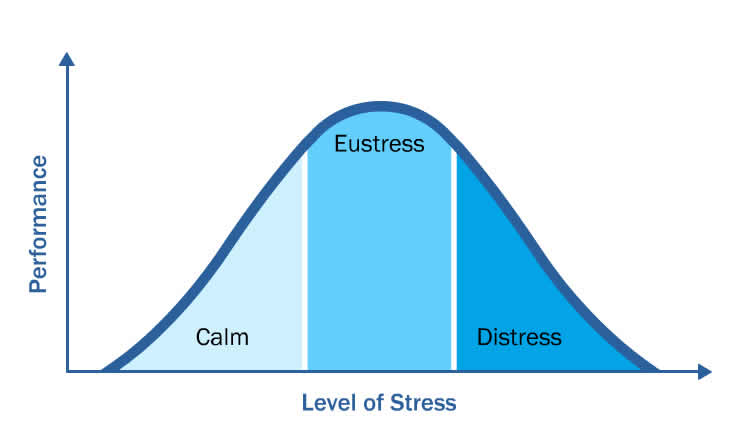
\includegraphics[width=0.6\linewidth]{chap1/images/def_stress.jpg}
  \caption[Stress level with Performance factor]{level of Stress with Performance factor.\index{Hasnain}}
  \label{fig:test1}
\end{figure}

\textbf{Acute Stress}

Fight or flight.  The body prepares to defend itself. It takes about 90 minutes for the metabolism to return to normal when the response is over.

\textbf{Chronic Stress}

The cost of daily living: bills, kids, jobs…This is the stress we tend to ignore or push down.  Left uncontrolled this stress affects your health- your body and your immune system.

\textbf{Eustress}

Stress in daily life that has positive connotations such as:
Marriage
Promotion
Baby
Winning Money
New Friends
Graduation

\textbf{Distress}

Stress in daily life that has negative connotations such as:
Divorce
Punishment
Injury
Negative feelings
Financial Problems
Work Difficulties

\subsection{Workplace Stress}

%\section{Problems and challenges} % actual problem statement

We hear a lot about stress, but what is it? As stated by the Canadian Mental Health Association: 


    “Stress is a reaction to a situation – it isn't about the actual situation. We usually feel stressed when we think that the demands of the situation are greater than our resources to deal with that situation. For example, someone who feels comfortable speaking in public may not worry about giving a presentation, while someone who isn't confident in their skills may feel a lot of stress about an upcoming presentation. Common sources of stress may include major life events, like moving or changing jobs. Long-term worries, like a long-term illness or parenting, can also feel stressful. Even daily hassles like dealing with traffic can be a source of stress.”

    From: “Stress”, Canadian Mental Health Association, 2018


\begin{table*}\centering
\ra{1.3}
\begin{tabular}{@{}rrrrcrrr@{}}\toprule
& \multicolumn{3}{c}{$w = 8$} & \phantom{abc}& \multicolumn{3}{c}{$w = 16$} \\
\cmidrule{2-4} \cmidrule{6-8} 
& $t=0$ & $t=1$ & $t=2$ && $t=0$ & $t=1$ & $t=2$\\ \midrule
$dir=1$\\
$c$ & 0.0790 & 0.1692 & 0.2945 && 0.3670 & 0.7187 & 3.1815\\
$c$ & -0.8651& 50.0476& 5.9384&& -9.0714& 297.0923& 46.2143\\
$c$ & 124.2756& -50.9612& -14.2721&& 128.2265& -630.5455& -381.0930\\
$dir=0$\\
$c$ & 0.0357& 1.2473& 0.2119&& 0.3593& -0.2755& 2.1764\\
$c$ & -17.9048& -37.1111& 8.8591&& -30.7381& -9.5952& -3.0000\\
$c$ & 105.5518& 232.1160& -94.7351&& 100.2497& 141.2778& -259.7326\\
\bottomrule
\end{tabular}
\caption{A Beautiful and Complex Table}\label{tab:sometable}
\end{table*}



\subsection{Mental Stress disorder and disabilities}
\subsection{Workplace Stress become anxiety}
\subsection{Stress management}
\section{Motivation}

\section{Goal and contribution} 
\blindtext

\begin{figure}[ht!] % supposedly places it here ...
  \centering
  
\includegraphics[width=0.6\linewidth]{test_image_goku}
  \caption[This is the short caption for List of Figures]{A test figure.  This caption is huge, but in the list of figures only the smaller version in the square brackets will appear.\index{Goku il-king}}
  \label{fig:test12}
\end{figure}

A test figure is shown in Figure~\ref{fig:test1}.

\subsection{Research Goal}

\begin{figure}[!ht]
    \centering
    \subbottom[Goku]{
\includegraphics[width=0.3\textwidth]{test_image_goku}}\qquad
    \subbottom[More Goku]{
\includegraphics[width=0.3\textwidth]{test_image_goku}}%
    \caption[Short Caption]{The same super saiyan. Two times.}        
    \label{fig:test2}
\end{figure}

Two figures shown side by side are shown in Figure~\ref{fig:test2}.

\subsection{Research Questions and Hypothesis}


In the early nineties, \acs{GSM} was deployed in many European countries. \ac{GSM} offered for the first time international roaming for mobile subscribers. The \acs{GSM}’s use of \ac{TDMA} as its communication standard was debated at length. And every now and then there are big discussion whether \ac{CDMA} should have been chosen over \ac{TDMA}.

If you want to know more about \acf{GSM}, \acf{TDMA}, \acf{CDMA} and other acronyms, just read a book about mobile communication. Just to mention it: There is another \ac{UA}, for testing.

\section{Structure of the Thesis}

